% PHSS thesis. Structure follows the supplied reference; project prose is original.
\documentclass[a4paper,12pt]{report}
\usepackage[margin=0.8in]{geometry}
\usepackage[T1]{fontenc}
\usepackage[utf8]{inputenc}
\usepackage{lmodern,amsmath,amssymb,graphicx,setspace,booktabs,float,array,longtable}
\usepackage[english]{babel}
\usepackage[autostyle,english=american]{csquotes}
\usepackage[font=small]{caption}
\usepackage{cite,url,xcolor,tikz}
\usetikzlibrary{arrows.meta,positioning,fit,backgrounds}
\usepackage[hidelinks]{hyperref}
\onehalfspacing
\emergencystretch=3em
\setlength{\tabcolsep}{4pt}
\renewcommand{\arraystretch}{1.15}
\renewcommand{\topfraction}{0.9}
\renewcommand{\bottomfraction}{0.8}
\renewcommand{\textfraction}{0.08}
\renewcommand{\floatpagefraction}{0.65}
\setcounter{totalnumber}{4}
\graphicspath{{figures/}}
\newcolumntype{P}[1]{>{\raggedright\arraybackslash}p{#1}}
\newcommand{\module}[1]{{\small\path{#1}}}
% Replace these fields with confirmed team and institutional details.
\newcommand{\ProjectTitle}{CACM-PHSS: A Multi-Agent Personalized Hybrid Study System}
\newcommand{\TeamNames}{Sreevalliputhuru Siri Priya (CB.AI.U4AID23039), Smera S Kini (CB.AI.U4AID23043), Penneru Shaswathi Sanjana (CB.AI.U4AID23066) and Kesarla Hasini Srinilaya (CB.AI.U4AID23067)}
\newcommand{\GuideName}{[Thesis advisor name]}
\newcommand{\DeanName}{[Head of department / authorised signatory]}
\newcommand{\DepartmentName}{Department of Artificial Intelligence}
\newcommand{\UniversityName}{Amrita Vishwa Vidyapeetham}
\newcommand{\CampusName}{Coimbatore Campus (India)}
\newcommand{\DegreeName}{BACHELOR OF TECHNOLOGY}
\newcommand{\ProgrammeName}{ARTIFICIAL INTELLIGENCE AND DATA SCIENCE}
\newcommand{\SubmissionMonth}{October 2026}
\newcommand{\ExamDate}{[Examination date]}
\newcommand{\PlaceName}{Coimbatore}

\newcommand{\TeamTitleRows}{SREEVALLIPUTHURU SIRI PRIYA (CB.AI.U4AID23039)\\[0.15cm]SMERA S KINI (CB.AI.U4AID23043)\\[0.15cm]PENNERU SHASWATHI SANJANA (CB.AI.U4AID23066)\\[0.15cm]KESARLA HASINI SRINILAYA (CB.AI.U4AID23067)}

\hypersetup{pdftitle={CACM-PHSS: A Multi-Agent Personalized Hybrid Study System},pdfauthor={PHSS project team}}
\begin{document}
\hypersetup{pageanchor=false}\pagenumbering{gobble}
\thispagestyle{empty}
\begin{large}
\begin{center}
{\Large\bfseries\MakeUppercase{\ProjectTitle}\par}
\vspace{1cm}
A Thesis\\[0.2cm]
Submitted in partial fulfilment for the Degree of\\[0.2cm]
\textbf{\DegreeName}\\[0.2cm]
in\\[0.2cm]
\textbf{\ProgrammeName}\\[0.8cm]
by\\[0.3cm]
{\large\bfseries\TeamTitleRows}\\[0.7cm]
\vfill\IfFileExists{figures/institution-logo.png}{
\includegraphics[width=10.5cm]{institution-logo.png}}{\fbox{\parbox[c][1.7cm][c]{4.5cm}{\centering Institution logo\\to be supplied}}}
\vfill
\MakeUppercase{\DepartmentName}\\[0.2cm]
{\Large\bfseries\MakeUppercase{\UniversityName}}\\[0.2cm]
\CampusName\\[0.5cm]
\SubmissionMonth
\end{center}
\end{large}
\clearpage
\begin{center}
\DepartmentName\\
{\Large\bfseries\MakeUppercase{\UniversityName}}\\
\CampusName\\[1.7cm]
{\Large\bfseries BONAFIDE CERTIFICATE}
\end{center}
\vspace{0.7cm}
\noindent This is to certify that the thesis entitled \enquote{\ProjectTitle}, submitted by \TeamNames\ for the award of the \DegreeName\ degree in \ProgrammeName, is a record of the project work carried out under the guidance of \GuideName\ in \DepartmentName, \UniversityName.

\noindent\textit{Draft certificate: institutional wording, eligibility, names and signatures must be verified by the institution before submission.}
\vfill
\noindent Submitted for the examination held on \ExamDate.
\vfill
\noindent\textbf{INTERNAL EXAMINER}\hfill\textbf{EXTERNAL EXAMINER}
\vfill
\begin{center}\textbf{\GuideName}\\Thesis Advisor\\\DepartmentName\\\UniversityName\\\CampusName\end{center}
\clearpage
\begin{center}
\DepartmentName\\
{\Large\bfseries\MakeUppercase{\UniversityName}}\\
\CampusName\\[1.7cm]
{\Large\bfseries DECLARATION}
\end{center}
\vspace{0.7cm}
\begin{flushleft}We, \TeamNames, submit this thesis entitled \enquote{\ProjectTitle} as the account of the project implementation described in this document. The thesis distinguishes implemented features, externally published work, deterministic software verification and proposed future work. References are provided for the literature discussed.
\end{flushleft}

\noindent The project team must review the complete text, confirm its contribution statement and comply with the institution's originality and AI-assistance disclosure requirements before signing this declaration. Institutional declarations about prior submission must be added only after confirmation by the students.
\par\vspace{1cm}
\noindent\textbf{Place:} \PlaceName\\[0.4cm]\textbf{Student signatures:} \rule{5cm}{0.4pt}\\[0.4cm]
\textbf{Date:} \ExamDate
\vfill
\begin{center}\textbf{COUNTERSIGNED}\\[1.0cm]\textbf{\DeanName}\\\DepartmentName\\\UniversityName\end{center}

\clearpage
\pagenumbering{roman}\hypersetup{pageanchor=true}
\tableofcontents
\chapter*{Acknowledgements}
\addcontentsline{toc}{chapter}{Acknowledgements}
We thank our project advisor, \GuideName, for guidance during the development and review of this work. We also acknowledge the faculty and technical staff of \DepartmentName, \UniversityName, for their support.

We acknowledge the researchers and open-source communities whose work made the implementation possible. The project brings together web development, cognitive modelling, language-model services, academic retrieval and software testing. These foundations are identified in the references and in the implementation discussion.

We are grateful to the classmates, friends and family members who supported the project. The final names, institutional acknowledgements and signatures will be confirmed by the project team before submission.
\vspace{1cm}
\begin{flushright}\TeamNames\end{flushright}
\clearpage
\listoffigures
\addcontentsline{toc}{chapter}{List of figures}
\clearpage
\listoftables
\addcontentsline{toc}{chapter}{List of tables}
\clearpage
\chapter*{Abbreviations}
\addcontentsline{toc}{chapter}{Abbreviations}
\begin{longtable}{P{0.20\textwidth}P{0.73\textwidth}}
AI & Artificial Intelligence\\
API & Application Programming Interface\\
AST & Abstract Syntax Tree\\
BKT & Bayesian Knowledge Tracing\\
CACM & Cross-Agent Cognitive Modeling\\
DOCX & Office Open XML Word document format\\
DOI & Digital Object Identifier\\
HTTP & Hypertext Transfer Protocol\\
ITS & Intelligent Tutoring System\\
JSON & JavaScript Object Notation\\
LLM & Large Language Model\\
OCR & Optical Character Recognition\\
PDF & Portable Document Format\\
PHSS & Personalized Hybrid Study System\\
RAG & Retrieval-Augmented Generation\\
SQL & Structured Query Language\\
UI & User Interface\\
\end{longtable}
\clearpage
\chapter*{List of symbols}
\addcontentsline{toc}{chapter}{List of symbols}
\begin{longtable}{P{0.22\textwidth}P{0.71\textwidth}}
$u$ & Student profile identifier\\
$c$ & Normalised concept identity\\
$m_t$ & Estimated concept mastery before evidence event $t$\\
$q_t$ & Confidence indicator stored with the concept\\
$n_t$ & Number of accepted assessment attempts\\
$p_t$ & Performance recorded by the evaluator\\
$r_t$ & Reliability attached to the evidence\\
$d_t$ & Normalised activity difficulty used in evidence weighting\\
$w_t$ & Effective evidence weight\\
$E_{u,c}$ & Stored assessment evidence for student $u$ and concept $c$\\
$\Delta$ & Difference between two cross-agent performance values\\
$\tau$ & Conflict detection threshold\\
$\pi$ & Existing rule-based activity-selection policy\\
$P$ & Bounded ordered study plan\\
$i$ & Index of the current activity in the plan\\
\end{longtable}
\chapter*{Abstract}
\addcontentsline{toc}{chapter}{Abstract}
A student may understand an explanation, struggle to implement the same idea in code, and find it difficult to interpret a research paper about it. When these activities are handled by separate tools, their results rarely form a consistent picture of the student's needs. CACM-PHSS addresses this integration problem through a web-based Personalized Hybrid Study System with Learning, Coding and Research agents supported by Cross-Agent Cognitive Modeling.

The application uses a React and TypeScript interface, a FastAPI backend and profile-owned SQLite persistence. A common natural-language input initiates semantic routing and a bounded activity plan. The Learning Agent provides explanations and adaptive practice. The Coding Agent supplies Python exercises, evaluates original submissions and recommends follow-up practice. The Research Agent retrieves academic records, processes uploaded PDFs and creates reports from attributed source material. Shared assessment evidence supports mastery estimates, misconception tracking and diagnostics when observations disagree.

The main contribution is an implemented, inspectable control loop: observe the student state, select and plan an activity, invoke the relevant services, evaluate student work, save evidence and revise the next action. Generation and navigation are kept separate from mastery updates. Full-text excerpts and abstract-only sources remain labelled separately, and research reports preserve page or chunk provenance where available.

Software validation includes a recorded run of 77 backend tests, 34 executions in selected existing coding and persistence suites, and nine selected browser tests in the thesis-preparation rerun. These results establish tested workflow behaviour under controlled offline provider fixtures. They do not establish learning gains, calibrated mastery probabilities or unrestricted live-provider reliability. The system demonstrates bounded agentic coordination for personalised study while making its current educational, execution-security and source-coverage limits explicit.

\clearpage
\pagenumbering{arabic}
\chapter{Introduction}\section{Background}
Personalised learning involves more than changing the wording of an explanation. A useful study system must notice what a student can do, distinguish an untested assumption from assessed understanding, and choose a suitable next activity. This becomes difficult when the student moves between conceptual learning, programming and research reading. Each activity reveals a different aspect of understanding, yet ordinary tools often store these observations independently.

Consider a student studying recursion. The student may explain a base case correctly in a short answer but write a function that never terminates. A lesson-only tool may conclude that the topic is understood, while a programming tool sees only the failed program. Neither observation should be discarded. The disagreement is useful evidence that further checking is needed. PHSS was developed around this practical problem: connecting educational activities without treating every generated response or visited screen as a learning achievement.

Large language models make it possible to interpret natural requests and prepare varied explanations. However, a language model response alone does not provide a reliable learning record. The surrounding application must decide which services may act, validate their outputs, retain evidence and recover when an external service fails. The design therefore combines language-model capabilities with explicit software policies and persistent state.

\section{Motivation}
The immediate motivation was to create a single study environment in which a student can ask for help naturally and continue into the appropriate activity. The student should be able to request a lesson, a programming exercise or academic papers without first understanding the internal organisation of the software. The same environment should retain a student's previous assessed work and use it when deciding what to offer next.

A second motivation concerns trust. An attractive dashboard can be misleading if it treats activity counts as mastery. A research report can appear complete while containing details that were never present in its sources. A code correction can look convincing without having been executed. These risks shaped the project requirements. The implementation separates assessed student responses from system-generated material and displays the coverage of its evidence.

The application was initially exercised through a Streamlit prototype. The current work presents the subsequent web application, which reuses the Python service architecture through a React interface and FastAPI endpoints. Streamlit is relevant to the development history, but it is not the primary application evaluated or described in this thesis.

\section{Problem Statement}
The project addresses the following engineering problem: how can one web application coordinate learning, coding and research activities using a shared student model, while preserving the identity, provenance and limitations of the evidence produced by each workflow?

This problem has several connected parts. Natural-language requests must enter actual workflows rather than produce generic conversational answers. Cognitive state must be updated only after a supported assessment. Unfinished work must survive browser refresh and application restart. Research material must retain its source coverage. Failures must leave a recoverable state rather than a misleading success screen. The implementation must also remain understandable enough to demonstrate to students and faculty.

\section{Objectives}
The first objective is to provide a common entry point that interprets a student's request and selects one or more appropriate specialist activities. The second is to maintain a shared, profile-specific cognitive record that can be read by all three agents. The third is to make adaptation visible through practice difficulty, focused feedback, diagnostics and follow-up recommendations.

A further objective is to integrate real tools: question generation and assessment, controlled Python execution, academic retrieval, PDF extraction and document export. These actions must have explicit limits and observable outcomes. Finally, the system must preserve work through persistence and provide deterministic tests for important workflows and failure cases.

\section{Contributions}
The project contribution is an integrated application and its supporting control mechanisms. It does not introduce a newly trained foundation model or claim a new statistical estimator of human knowledge. Its main contributions are summarised in Table~\ref{tab:contributions}.

\begin{table}[htbp]\centering\small
\caption{Implemented project contributions}\label{tab:contributions}
\begin{tabular}{P{0.26\textwidth}P{0.66\textwidth}}\toprule
Contribution & Implemented meaning\\\midrule
Unified orchestration & Natural-language routing into real Learning, Coding and Research workflows with bounded plans.\\
Shared cognitive evidence & Common concept identities, mastery estimates, misconception records and cross-agent conflict handling.\\
Assessment boundaries & Lessons, searches, uploads, report generation and AI corrections do not count as student mastery.\\
Adaptive practice & State-aware questions and coding recommendations using existing inspectable policies.\\
Grounded research support & Persistent collections, extracted PDF content, source-linked claims and coverage-aware report export.\\
Recoverable operation & Profile-owned state, duplicate assessment protection, checkpoints and explicit retry paths.\\\bottomrule
\end{tabular}
\end{table}

These contributions are strongest when considered together. For example, saving a code draft is useful on its own, but saving the draft, its assessment receipt, the active activity and the recommendation context makes the next interaction coherent. The project focuses on this continuity between actions.

\section{Scope}
The implemented application is intended for local educational use and demonstrations. The student interface supports lessons and adaptive quizzes, Python coding practice, standalone code review, academic search, uploaded PDF analysis and research-report export. Direct agent buttons provide an alternative entry to the same underlying services. They do not form separate implementations of the agents.

The current system uses local profiles rather than production user authentication. Its controlled code runner is not a hardened security sandbox. It processes machine-readable PDF text and does not implement OCR. The cognitive policies are rule-based, and their thresholds have not been calibrated through a real-student study. These limits define the scope of the contribution rather than invalidate the implemented workflows.

\section{Organisation of the Thesis}
Chapter~2 reviews relevant work in student modelling, agentic interaction, program evaluation and source-grounded generation. Chapter~3 introduces the application architecture and formalises its state and evidence model. Chapter~4 explains the agentic control loop and recovery strategy. Chapter~5 describes the Learning and Coding agents. Chapter~6 describes research retrieval, PDF analysis and grounded reporting. Chapter~7 presents recorded software verification and its limits. Chapter~8 concludes the work and separates completed features from future research. The appendix records implementation parameters and reproduction guidance.

\chapter{Literature Review and Research Gap}\section{Introduction}
The project draws on several areas that are often studied separately: intelligent tutoring, student modelling, language-model agents, automated programming support and retrieval-based writing. The purpose of this review is to explain the design choices that these areas motivate. It is not a claim that PHSS reproduces every reviewed algorithm or outperforms the systems in the literature.

The review uses identifiable primary papers and distinguishes their published contributions from the application's own implementation. No performance number from another paper is reused as a PHSS result. This distinction is especially important because the present evaluation concerns software behaviour, whereas educational studies may measure learning outcomes over extended periods.

\section{Student Modelling and Knowledge Tracing}
Corbett and Anderson describe knowledge tracing as maintaining estimates of procedural knowledge while a student works through programming tasks~\cite{corbett1994}. Their work establishes a useful principle for this project: the next learning action can depend on an evolving student model rather than a fixed sequence alone. PHSS applies this principle through concept-level assessment records. Its weighted update is not the Bayesian Knowledge Tracing model described in that paper.

Piech and colleagues investigate recurrent neural networks for modelling sequences of student interactions~\cite{piech2015}. Their work represents a data-driven direction in knowledge tracing. In contrast, PHSS uses explicit rules and does not train a recurrent knowledge-tracing model. This choice keeps decisions inspectable in a project with no collected student-training dataset, while limiting claims about predictive accuracy.

The practical lesson from these works is that a student model should have a defined connection to observed performance. PHSS therefore separates an initial neutral estimate from demonstrated competence. An initial mastery value of 0.5 is a software prior, not a statement that a new student already knows half of a topic.

\section{Intelligent Tutoring and Educational Validation}
Kulik and Fletcher review controlled evaluations of intelligent tutoring systems~\cite{kulik2016}. Such work matters because a technically functioning tutor and an educationally effective tutor are different claims. A system may save state correctly and still provide explanations that students find difficult to use. Conversely, a promising lesson design may fail operationally if student work is lost.

For PHSS, this distinction leads to a restrained evaluation strategy. Deterministic tests check routing, persistence, assessment boundaries and recovery. They cannot establish learning gains, long-term retention, engagement or the calibration of mastery estimates. Those outcomes require an appropriately designed student study. The thesis therefore reports engineering validation and leaves educational validation as future work.

\section{Reasoning and Acting in Language-Model Systems}
ReAct studies the interleaving of reasoning-related steps and actions that obtain information from an external environment~\cite{yao2022}. Its relevance to PHSS is the separation between producing text and taking an action whose result can influence subsequent behaviour. In the application, examples of observable actions include loading an exercise, running supplied tests and extracting a PDF chunk. PHSS does not claim to reproduce ReAct's benchmark protocol or expose an unrestricted language-model reasoning trace.

AutoGen presents an infrastructure for applications in which configurable agents interact through conversation and tools~\cite{wu2023}. It illustrates a general approach to assigning specialised roles. PHSS implements its own Python coordination and state-sharing services; it does not depend on AutoGen as its runtime. The comparison is architectural: specialist responsibilities and explicit interaction rules help prevent a multi-agent label from becoming merely a collection of differently named chat prompts.

\section{Feedback and Iterative Refinement}
Self-Refine explores improving generated outputs through repeated feedback and revision without additional model training~\cite{madaan2023}. The relevant design idea is that an initial output need not be accepted without checking. PHSS applies bounded generate-and-check behaviour to coding packages and separates original student code from an AI-proposed correction. It does not assume that self-feedback alone proves correctness.

This distinction is visible in the coding workflow. A revised solution may pass the supplied tests while still failing an untested input. A generated task and its generated reference solution may also share an error. Accordingly, the system labels the scope of verification and avoids treating an AI-written correction as student achievement.

\section{Functional Evaluation of Generated Programs}
Chen and colleagues use executable tasks to investigate functional correctness in code generation~\cite{chen2021}. For PHSS, the useful connection is the role of behaviour-based checking alongside language-model feedback. The application executes supplied function tests for assessed practice and records their individual outcomes. It does not evaluate its model on HumanEval or claim the paper's benchmark results.

The project also supports a separate standalone review mode. In that mode, there may be no trusted behavioural specification or tests. Syntax inspection and AI suggestions can be helpful, but they cannot support the same correctness claim as an executed exercise contract. Keeping these workflows separate avoids an important source of overstatement.

\section{Retrieval and Source-Grounded Generation}
Lewis and colleagues introduce retrieval-augmented generation by combining retrieved information with a generative model for knowledge-intensive tasks~\cite{lewis2020}. The broader motivation is relevant to the Research Agent: a report should be connected to source material rather than rely entirely on model memory. PHSS uses retrieved abstracts and uploaded PDF excerpts, with preserved source identity and page or chunk references. It is not a trained implementation of the original RAG architecture.

Source access is only one part of grounded reporting. The application must also distinguish an author's reported finding, a saved AI interpretation and a proposed research direction. An absent dataset name must remain absent. A complete-looking section should not be created by guessing from a paper title. These requirements shaped the conservative report writer described in Chapter~6.

\section{Summary of Reviewed Work}
Table~\ref{tab:literature} summarises the specific design relevance of the reviewed publications. The comparison describes conceptual relationships, not a common benchmark or a ranking of systems.
\begin{table}[htbp]\centering\small
\caption{Literature relationships and project boundaries}\label{tab:literature}
\begin{tabular}{P{0.25\textwidth}P{0.31\textwidth}P{0.35\textwidth}}\toprule
Work & Relevant idea & PHSS boundary\\\midrule
Knowledge tracing~\cite{corbett1994} & Evolving student estimates & Uses a different explicit update rule.\\
Deep Knowledge Tracing~\cite{piech2015} & Interaction-sequence modelling & No trained recurrent student model.\\
ITS review~\cite{kulik2016} & Controlled educational evaluation & Current results are software tests.\\
ReAct~\cite{yao2022} & Action results inform later steps & Bounded application control, not benchmark replication.\\
AutoGen~\cite{wu2023} & Specialised agents and tools & Own coordinator; no AutoGen runtime.\\
Self-Refine~\cite{madaan2023} & Feedback and revision & Validation remains limited and explicit.\\
Code evaluation~\cite{chen2021} & Executable functional tests & Supplied task tests, not HumanEval evaluation.\\
RAG~\cite{lewis2020} & Retrieved source grounding & Excerpt-based provenance, not RAG training.\\\bottomrule
\end{tabular}
\end{table}

\section{Research Gap and Project Position}
The engineering gap addressed here is the continuity between learning activities. A student needs more than three isolated interfaces: evidence from a lesson assessment should remain available when coding begins, and research understanding should be assessed separately from the system's ability to summarise a paper. Operational details such as duplicate protection and refresh recovery are necessary for that continuity.

PHSS offers an implementation of this integrated approach. The gap statement is limited to the application's design problem; it does not assert that no prior educational system has combined multiple activities. The defensible contribution is the implemented coordination, evidence boundaries, source-aware reporting and testable recovery behaviour in this particular project.

\chapter{System Model and Problem Formulation}\section{Introduction}
PHSS is organised as a browser interface around reusable Python services. The application separates presentation, orchestration, specialist actions, cognitive evidence and storage. This separation matters because a user-interface transition must not silently become a learning assessment. It also allows the common query input and direct agent buttons to enter the same workflows.

The deployed local application serves the compiled frontend and API from a FastAPI process. React and TypeScript manage the visible workspace. FastAPI validates requests and calls the application service, which loads a profile-owned state snapshot and invokes the existing Python modules. SQLite stores supported state and research material. External language-model and academic-search services remain outside this persistence boundary.

\section{Overall Architecture}
Figure~\ref{fig:architecture} shows the main relationships. CACM is a shared cognitive layer, not a fourth specialist agent. The agents communicate through structured outputs, shared services and stored evidence rather than through an unrestricted conversation between independent chatbots.

\begin{figure}[htbp]\centering
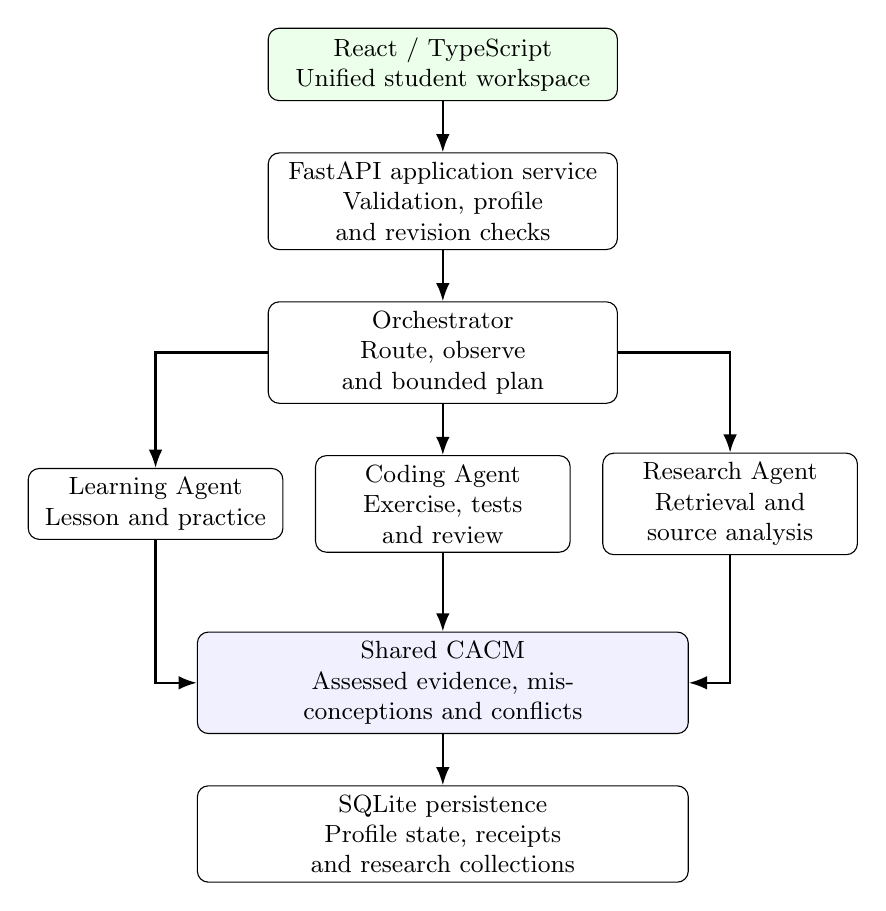
\begin{tikzpicture}[node distance=0.65cm and 0.4cm,box/.style={draw,rounded corners,align=center,font=\small,minimum height=0.9cm,text width=4.2cm},arr/.style={-{Latex},thick}]
\node[box,fill=green!8](ui){React / TypeScript\\Unified student workspace};
\node[box,below=of ui](api){FastAPI application service\\Validation, profile and revision checks};
\node[box,below=of api](orch){Orchestrator\\Route, observe and bounded plan};
\node[box,below=of orch,text width=3.0cm](code){Coding Agent\\Exercise, tests and review};
\node[box,left=of code,text width=3.0cm](learn){Learning Agent\\Lesson and practice};
\node[box,right=of code,text width=3.0cm](research){Research Agent\\Retrieval and source analysis};
\node[box,below=1.0cm of code,text width=6.0cm,fill=blue!6](cacm){Shared CACM\\Assessed evidence, misconceptions and conflicts};
\node[box,below=of cacm,text width=6.0cm](db){SQLite persistence\\Profile state, receipts and research collections};
\draw[arr](ui)--(api);\draw[arr](api)--(orch);
\draw[arr](orch)--(code);\draw[arr](orch)-|(learn);\draw[arr](orch)-|(research);
\draw[arr](code)--(cacm);\draw[arr](learn)|-(cacm);\draw[arr](research)|-(cacm);
\draw[arr](cacm)--(db);
\end{tikzpicture}
\caption{Application architecture. Agent-to-CACM arrows denote assessed evidence; ordinary content generation does not update mastery.}\label{fig:architecture}
\end{figure}

\section{Responsibilities of the Main Layers}
The frontend owns navigation, input controls, the embedded editor and rendering of returned state. It shows the active agent, but the student does not have to select one before asking a question. The backend service owns the connection between a request and a real workflow. The orchestrator interprets intent, identifies a concept, reads cognitive observations and prepares the bounded sequence.

Each agent supplies domain-specific behaviour. The Learning Agent prepares explanations, questions and feedback. The Coding Agent prepares tasks, assesses original submissions and chooses follow-up practice. The Research Agent retrieves academic records and analyses available source material. Their integration adapters translate supported assessment outcomes into the common evidence format. The central cognitive engine validates ownership, records evidence, updates estimates and detects disagreement.

\section{Student and Concept State}
For a profile $u$ and concept $c$, the state can be described as
\begin{equation}
S_{u,c}=(m,q,n,H,E,A),
\end{equation}
where $m$ is estimated mastery, $q$ is the confidence indicator, $n$ is the accepted-attempt count, $H$ contains misconception hypotheses, $E$ denotes assessment evidence and $A$ represents active conflicts. This notation summarises the implemented objects; it is not an additional trained model.

The code initialises a previously unseen concept with mastery 0.5, confidence 0 and zero attempts. Policies explicitly check the absence of attempts, so the neutral prior does not justify advanced practice. Concept normalisation reduces accidental separation caused by case or recognised aliases. It is not a universal semantic ontology: unrelated or differently phrased concepts cannot always be assumed equivalent.

Misconception hypotheses retain more information than a plain error label. They can record support, contradiction, status and source agents. This allows the system to distinguish a confirmed concern from a hypothesis that still needs verification. A displayed misconception remains an inference from evaluated work, not a clinical or permanent judgement about the student.

\section{Assessment Evidence}
The common evidence object includes the student identifier, concept name, source agent, evidence type, performance, normalised difficulty, reliability, detected misconceptions, timestamp and evidence identifier. Numeric inputs are validated, and the cognitive engine checks that the evidence belongs to the student whose model is being updated.

This structure is the main communication contract between specialist assessment and CACM. A question evaluator and a coding evaluator do not have to return identical domain-specific feedback. They must provide a supported assessment that can be adapted into this common contract. Source-agent identity remains available so that later conflict detection can compare observations from different activities.

Table~\ref{tab:evidence-boundary} records the boundary used throughout the application. It prevents the system's own productivity from being confused with a student's learning.
\begin{table}[htbp]\centering\small
\caption{Actions and their relationship to mastery evidence}\label{tab:evidence-boundary}
\begin{tabular}{P{0.53\textwidth}P{0.38\textwidth}}\toprule
Action & Creates mastery evidence?\\\midrule
Open a lesson or navigate to another activity & No\\
Generate a question without answering it & No\\
Submit a supported learning answer for evaluation & Yes, through the assessment path\\
Run an original coding submission through assessment & Yes, after accepted evaluation\\
Obtain an AI correction or test that correction & No student mastery credit\\
Search papers, upload PDFs or analyse source excerpts & No\\
Export a research report & No\\
Submit an evaluated research-comprehension answer & Yes, through the assessment path\\
Start recommended coding practice & No\\\bottomrule
\end{tabular}
\end{table}

\section{Implemented Mastery Update}
The mastery engine applies a bounded weighted update. For an accepted evidence event, its effective weight is
\begin{equation}\label{eq:weight}
w_t=r_t\left(0.5+0.5d_t\right).
\end{equation}
The updated mastery is
\begin{equation}\label{eq:mastery}
m_{t+1}=\operatorname{clip}_{[0,1]}\left(m_t+w_t(p_t-m_t)\right).
\end{equation}
The implementation rounds the stored mastery to three decimal places. It increases the attempt count by one and updates confidence as
\begin{equation}\label{eq:confidence}
q_{t+1}=\min\left(1,q_t+0.1w_t\right),
\end{equation}
again storing a rounded value. These equations describe the code in \module{app/cognitive/mastery_engine.py}.

For illustration, if $m_t=0.5$, $p_t=1$, $r_t=0.8$ and $d_t=0$, then $w_t=0.4$ and the resulting mastery is 0.7. This is an arithmetic example, not a measured student result. It also explains why the current coding policy can move directly from easy to hard after sufficiently strong evidence: the policy reads the updated estimate rather than requiring a fixed one-level transition.

Confidence in Equation~\ref{eq:confidence} is an accumulating software indicator. It is not a calibrated probability that the student has mastered the topic. Its monotonic increase with accepted evidence is a limitation worth stating because repeated observations do not necessarily make a pedagogical judgement correct.

\section{Cross-Agent Conflict Model}
Conflict detection compares evidence for the same student and normalised concept when the source agents differ. The performance difference is
\begin{equation}
\Delta=|p_a-p_b|.
\end{equation}
With the default detector, a difference below 0.35 is not flagged. A difference of at least 0.35 produces a conflict, and at least 0.60 is classified as high severity. These are configured engineering thresholds, not empirically validated educational cut-offs.

The resulting conflict does not prove that either agent is wrong. A conceptual question and a programming exercise can demand different abilities. The application uses the discrepancy to request focused diagnostic evidence and temporarily restrict normal progression. This is a more cautious response than hiding the disagreement inside an average.

\section{Bounded Study Plan}
A workspace plan contains a profile owner, request identifier, original query, concept, ordered steps and current index. Supported steps are Learning, Coding and Research. Validation limits the sequence to the supported agent set and prevents repeated agent entries in the same bounded plan. The plan is therefore not an unrestricted autonomous task graph.

Each step records whether it has been prepared, its status, a baseline evidence count and any recoverable error. The distinction between \textit{assessed} and \textit{visited without assessment} is important. Advancing to another screen can finish a navigation step, but it does not establish understanding. A new accepted assessment after the step baseline is needed for the assessed label.

\section{Persistence Model}
The SQLite store contains profile records, revisioned state snapshots, research documents, academic-source records, search sessions and report preferences. Recovery reconstructs supported Python state through explicit codecs and session adapters. Assessment receipts help identify work that was already applied to CACM.

A browser profile selection is not authentication. Profile ownership checks prevent accidental cross-profile mixing in the supported local application, but they do not protect an exposed server from an unauthorised person who can access its APIs. This distinction informs the deployment scope in Chapter~7.

\section{Problem Formulation and Invariants}
The operational objective is to choose a useful next action from the current request, plan and evidence while preserving a small set of invariants. Evidence must belong to the active student. A repeated completed assessment must not increase mastery twice. Source coverage must remain visible. Provider failure must not invent a successful assessment. Refresh must recover committed work rather than create new evidence.

These requirements can be expressed as a state-transition constraint. If an operation does not accept a new evaluated student response, then the stored evidence set and mastery must remain unchanged by that operation. Testing this constraint is more informative than assigning an unsupported percentage of the application's code to ``agentic AI.''

\chapter{Proposed Methodology}\section{Overall Framework}
The methodology treats an educational request as the start of a stateful activity, not as a prompt that ends when a paragraph is generated. The application interprets the request, observes the relevant student state, creates a bounded plan and invokes the appropriate workflow. When the student responds, the assessment result can change the next action. Persistence connects these stages across separate browser requests.

The principal loop is shown in Figure~\ref{fig:loop}. The arrows represent application control and observable results. They do not imply that every stage is decided by a language model. Semantic routing and content generation use model services, whereas evidence validation, difficulty policies, revision checks and duplicate protection use explicit code.

\begin{figure}[htbp]\centering
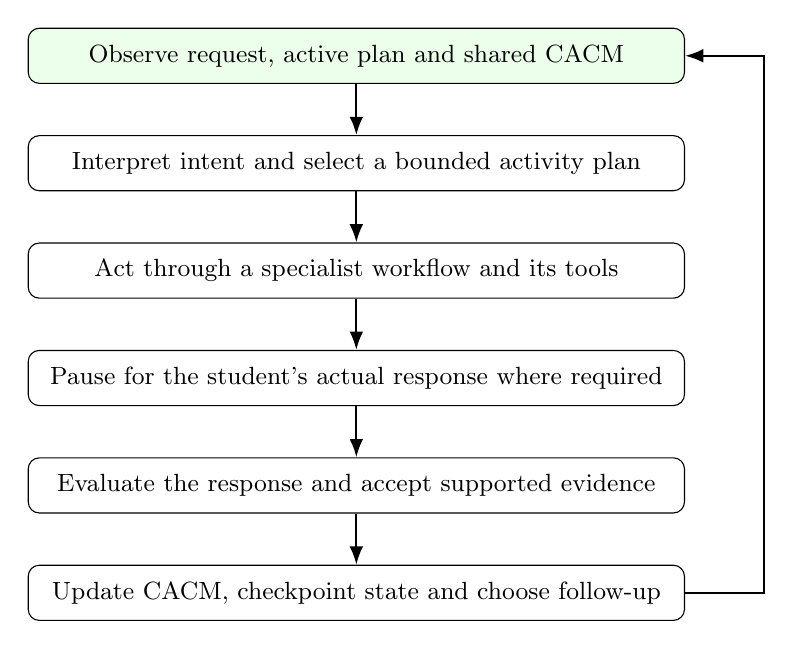
\begin{tikzpicture}[node distance=0.65cm,box/.style={draw,rounded corners,align=center,font=\small,text width=8.1cm,minimum height=0.7cm},arr/.style={-{Latex},thick}]
\node[box,fill=green!8](o){Observe request, active plan and shared CACM};
\node[box,below=of o](r){Interpret intent and select a bounded activity plan};
\node[box,below=of r](a){Act through a specialist workflow and its tools};
\node[box,below=of a](h){Pause for the student's actual response where required};
\node[box,below=of h](e){Evaluate the response and accept supported evidence};
\node[box,below=of e](u){Update CACM, checkpoint state and choose follow-up};
\draw[arr](o)--(r);\draw[arr](r)--(a);\draw[arr](a)--(h);\draw[arr](h)--(e);\draw[arr](e)--(u);
\draw[arr](u.east)--++(1,0)|-(o.east);
\end{tikzpicture}
\caption{Implemented agentic control loop with student interaction as an explicit boundary.}\label{fig:loop}
\end{figure}

\section{Natural-Language Entry and Semantic Routing}
The primary screen asks, ``What would you like help with today?'' A request is sent to the backend, where the existing query router produces a structured route. Its fields include the concept, selected agents, intent, reason and workflow mode. A coding request can select assessed practice or review of existing code. A research request can select academic search or the existing collection.

The primary router uses a language-model service to interpret meaning. A bounded local fallback is available for recognised explicit requests when semantic routing is unavailable. That fallback is a recovery measure rather than a replacement for the semantic architecture. It must not be described as evidence that every arbitrary request can be understood offline.

An ambiguous request can return a clarification question. The saved clarification is associated with the student profile and original request. This avoids choosing an unrelated task merely to show a result. The application also preserves the context needed to interpret a later clarification reply.

\section{Observation and Planning}
After routing, the orchestrator reads a concept observation from the shared student and cognitive engine. This includes assessed attempts, mastery and confidence estimates, misconception information and conflict status. The route and observation inform the bounded study sequence. A combined request such as learning a concept followed by coding practice can produce an ordered Learning--Coding plan.

Planning is distinct from execution. The system saves the plan before deferred provider work so that interruption does not erase its intent. Preparing a coding step binds the selected concept and exercise controls; preparing a research step binds the topic and collection/search mode. These operations do not themselves assess the student.

The present plan is deliberately limited. It does not schedule an arbitrary number of autonomous agents, execute indefinitely or complete student answers on the student's behalf. The bounded design makes progress, failure and recovery easier to inspect.

\section{Specialist Actions and Tool Boundaries}
Each specialist invokes services relevant to its task. Learning can request explanations, resource lookups and adaptive questions. Coding can load a verified exercise, validate a generated package and execute the student's original Python function against supplied tests. Research can retrieve actual academic records, extract PDF pages, analyse selected chunks and create a document.

These actions produce different kinds of output. A lesson is content. A test report is behavioural evidence with a defined contract. An academic abstract is a retrieved source with limited coverage. An exported report is a derived artifact. The integration layer preserves these distinctions rather than collapsing them into a single conversation transcript.

Tool invocation is also where important bounds are enforced. Input sizes, configured collection limits, candidate-generation attempts, execution timeouts and processing batches constrain work. When a bound prevents completion, the state remains explicit. A refusal or partial result is preferable to an invented complete result.

\section{Assessment, Evidence and Replanning}
The system pauses at points that require a genuine student response. A learning question waits for an answer; an exercise waits for original code; a research-comprehension activity waits for the student's interpretation. Assessment results enter their existing integration paths and may update CACM only after validation.

Replanning occurs through the existing policy services. Adaptive practice chooses a subsequent question using the updated state and session performance. Coding next-practice decisions use the original submission result and current cognitive model. A conflict can replace ordinary progression with a diagnostic requirement. These are bounded local revisions to the activity, not evidence of a general autonomous planner that can solve any educational goal.

The distinction is useful in demonstrations. The agentic behaviour is visible in a change of action justified by an observed result: a failed boundary-case test leads to revision guidance, or disagreement between conceptual and coding performance leads to diagnosis. Merely generating a new paragraph would not demonstrate that loop.

\section{Communication Between Agents and CACM}
The agents share the student's cognitive engine and model through Python service objects and persisted snapshots. They do not need direct access to each other's user-interface components. Learning and Coding evidence about the same normalised concept can be compared centrally, even though their original feedback formats differ.

This architecture also clarifies the meaning of ``multi-agent.'' The project contains specialised decision and workflow modules with distinct responsibilities, coordinated by an orchestrator. It does not require separate operating-system processes for each agent or a debate between multiple foundation models. The web frontend displays the results of those services through the same student interface.

\section{Checkpoints, Idempotency and Recovery}
Long operations are checkpointed at meaningful boundaries. For example, an assessment request can be recorded as pending before provider-dependent evaluation begins. If the process fails after local code execution but before the full assessment completes, the application can display the execution evidence separately and offer recovery without claiming a completed cognitive update.

Completed assessments have identifiers and receipts. An identical completed submission can return its cached result instead of changing mastery again. Snapshot revision checks detect a stale browser tab that attempts to overwrite newer state. These protections address different problems: duplicate work, interrupted work and competing saved versions.

The coding recommendation adds its own current-state token. When the student clicks the recommendation, the backend recomputes the decision. A token tied to an earlier submission or topic is rejected. This prevents a stale recommendation card from loading unrelated practice after the student has moved on.

\section{User Interface and Alternative Entry Paths}
The common input remains the primary route into the system. Three direct agent buttons provide a convenient way to demonstrate or start a specialist activity. Learning and Coding entry controls support both a topic list and a typed topic. The direct controls reuse the same backend workflows and shared state; they do not create separate private mastery models.

Lessons, the editor, academic search and collection controls appear within the study workspace. The active specialist is named so that the student can understand which workflow is handling the task. Supplementary structured details and topic controls use collapsed sections to avoid overwhelming the first view. The former professor-demo navigation was removed from the current application.

\section{Failure-Aware Operation and Performance}
The backend does not initialise every expensive workflow for every screen. In particular, Learning and Coding do not need to download research state simply to render. Independent learning-resource requests can run in parallel, while loading messages identify the operation that is still in progress. Timing headers support inspection of server work without inventing a performance improvement percentage.

External services can still be slow, unavailable or rate limited. Explicit retry actions, saved drafts and partial research statuses make those failures manageable. The project has not established a service-level latency guarantee, a high-concurrency deployment profile or a live-provider availability rate.

\section{Agentic Capability and Its Limits}
Table~\ref{tab:agentic-capabilities} connects the agentic terminology to concrete implementation behaviour. It avoids treating the entire web application as an autonomous model.
\begin{table}[htbp]\centering\small
\caption{Observable agentic capabilities in PHSS}\label{tab:agentic-capabilities}
\begin{tabular}{P{0.19\textwidth}P{0.42\textwidth}P{0.29\textwidth}}\toprule
Stage & Implemented behaviour & Boundary\\\midrule
Observe & Read concept evidence and current workflow & Stored estimates may be imperfect.\\
Interpret & Semantic route with structured modes & Ambiguity can require clarification.\\
Plan & Ordered, validated specialist steps & At most the supported bounded sequence.\\
Act & Invoke content, tests, retrieval and extraction & Tools operate within configured limits.\\
Evaluate & Assess actual student responses & AI-generated output earns no mastery.\\
Update & Save evidence and apply cognitive rules & No trained knowledge-tracing model.\\
Replan & Adapt questions, practice and diagnostics & Same-topic coding recommendations currently.\\\bottomrule
\end{tabular}
\end{table}

The result is a hybrid agentic system: model-assisted interpretation and generation operate inside a deterministic application control structure. This is a defensible description of what the project does. Claiming that all decisions are autonomous, that all agents continuously self-improve or that the system has been educationally calibrated would go beyond the implementation.

\chapter{Learning and Coding Agent Implementation}\section{Introduction}
The Learning and Coding agents share concept evidence but address different educational actions. Learning supports explanation and conceptual practice. Coding checks the student's ability to express an idea as executable Python. A shared model allows their observations to interact without pretending that a good verbal answer and a correct program are the same skill.

Both agents are accessible through the common natural-language input and direct buttons. The available topic lists are starting suggestions rather than the complete set of possible requests. Students can type a topic when it is not listed. Custom coding topics require successful bounded package generation and are not guaranteed to produce a usable exercise in every case.

\section{Learning Agent Workflow}
A learning request enters the existing learning runtime with the selected concept and shared student state. The service prepares an explanation and available educational resources. The interface presents the lesson within the same study workspace, together with practice and topic controls. Optional details remain collapsed until opened.

The learning workflow is state-aware. Prior assessed performance, confidence and misconception hypotheses can influence the kind of help requested. The generated explanation is content for the student to study; it is not a completed assessment. The system does not increase mastery because a lesson was displayed, because a link was opened or because the student continued to another activity.

A study-planning service also uses recorded concept information and configured topic relationships to suggest useful work. These suggestions are inspectable recommendations. They should not be presented as a learned optimal curriculum or proof that prerequisites have been mastered.

\section{Adaptive Questions and Difficulty Control}
When the student starts practice, the backend creates or resumes a topic-specific practice session. The question-generation service receives a difficulty and misconception target selected by the existing practice policy. The language model produces content that follows this decision; it does not have unrestricted authority to choose the difficulty.

The first question uses the current cognitive state. An unassessed concept starts with an easy question. Known misconceptions can require foundational work, while an uncertain hypothesis can require verification. Later questions use the latest session attempt as well as CACM. A fully incorrect answer maintains the current difficulty and probes the observed weakness. A partially correct answer also maintains difficulty to collect stronger evidence. A correct answer may increase difficulty by at most one level, subject to the mastery guardrail.

This is the implemented within-session learning policy, not the coding policy. The two should not be described as identical. In particular, the Coding Agent's state thresholds can produce a larger difficulty change, whereas the adaptive learning session explicitly limits an upward step to one level.

\begin{table}[htbp]\centering\small
\caption{Adaptive learning decisions within an active practice session}\label{tab:learning-policy}
\begin{tabular}{P{0.37\textwidth}P{0.54\textwidth}}\toprule
Latest observation & Policy response\\\midrule
No session attempt yet & Select from current CACM; no assessed history starts easy.\\
Performance equals zero & Keep the level; target observed weaknesses.\\
Performance strictly between zero and one & Keep the level and collect more evidence.\\
Performance reaches full correctness & Increase by at most one level unless the mastery guardrail prevents it.\\
Known or uncertain misconception & Include relevant verification or remediation targets.\\\bottomrule
\end{tabular}
\end{table}

\section{Topic-Specific Practice and Recovery}
A later refinement addressed a practical interface error: changing the lesson topic could leave the previous topic's question visible. The web service now binds visible practice to the active concept and preserves separate unfinished sessions. The current question's difficulty is displayed explicitly. Returning to a topic can restore its supported unfinished session rather than attach its question to a different lesson.

Question identifiers and assessment records provide a stable connection between a submitted answer and the question that was actually asked. A repeated completed answer does not create duplicate evidence. Refresh recovery restores the question and its saved state; it is not an instruction to generate a fresh question automatically.

Figure~\ref{fig:learning-ui} shows a direct browser capture of the implemented learning workspace. The profile and content in this figure are controlled fixtures, not records from a student experiment.
\begin{figure}[htbp]\centering
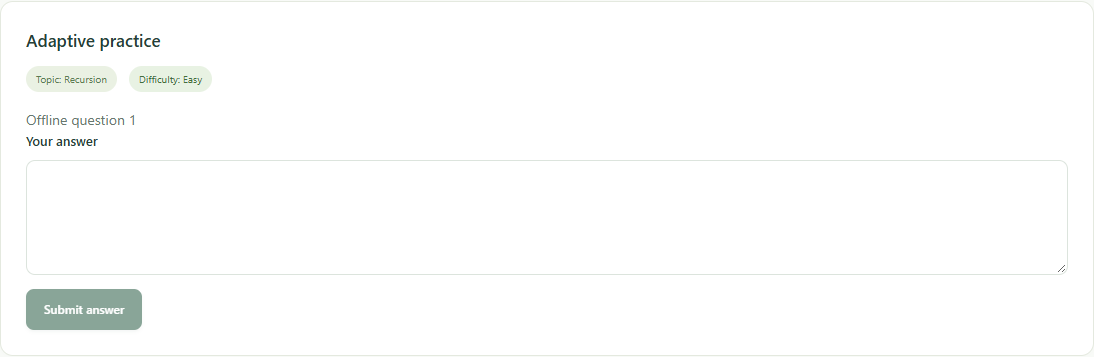
\includegraphics[width=0.98\textwidth,keepaspectratio]{learning-practice-detail.png}
\caption{Detail of topic-bound adaptive practice and an explicit difficulty label. Synthetic offline fixture.}\label{fig:learning-ui}
\end{figure}

\section{Coding Agent: Exercise Selection}
A request for practice loads a Python exercise chosen using the current concept state. The verified catalogue contains Recursion, Prime Numbers, Arrays, Strings, Python Functions and Searching Algorithms, with supported difficulty variants. For a topic outside this catalogue, the existing generator attempts to produce a structured task package and validates it before publication.

The initial coding decision is not random. If the student has no assessed attempts for the topic, or a known misconception needs remediation, the policy selects easy foundational practice. An uncertain misconception can select medium verification. Otherwise, mastery below 0.40 selects easy, mastery below 0.70 selects medium, and mastery at or above 0.70 selects hard. At high mastery, confidence affects whether the reason is verification or advanced extension.

An active cross-agent conflict has priority over these ordinary rules. The agent requests a diagnostic action rather than continuing normal progression. Table~\ref{tab:coding-policy} records the policy order, which matters because the first applicable branch wins.
\begin{table}[htbp]\centering\small
\caption{Ordered Coding Agent selection policy}\label{tab:coding-policy}
\begin{tabular}{P{0.46\textwidth}P{0.44\textwidth}}\toprule
Condition checked & Action / difficulty\\\midrule
Active cross-agent conflict & Diagnostic coding action; normal next-practice start blocked.\\
No assessed attempts or known misconception & Foundational / easy\\
Uncertain misconception hypothesis & Verification / medium\\
Mastery below 0.40 & Foundational / easy\\
Mastery at least 0.40 and below 0.70 & Guided / medium\\
Mastery at least 0.70, confidence below 0.50 & Verification / hard\\
Mastery at least 0.70, confidence at least 0.50 & Advanced / hard\\\bottomrule
\end{tabular}
\end{table}

Because CACM is shared, assessed learning history can influence the first coding exercise on that concept. A new coding interaction is not necessarily the student's first assessed encounter with the topic. At the same time, simply reading a lesson cannot justify increasing the coding level.

\section{Generated Exercise Validation}
An open-topic package includes a task title, specification, difficulty, function signature, starter code, progressive hints, supplied tests and a reference solution. Validation checks structure and supported Python behaviour, then runs the package's reference solution against its tests. The web path bounds generation to two candidate attempts.

This process reduces obvious unusable packages, but its limits are important. The model may generate both the tests and the reference solution, so they may share the same misunderstanding. Passing those tests establishes consistency with the supplied contract, not independent proof that the task specification is scientifically or pedagogically ideal. The reference solution is not included in the public exercise response shown to the student.

Only Python function-based practice is supported by this path. Unsupported language requests are not silently executed as another language. Code execution is bounded, but it is intended for trusted local use rather than hostile public submissions.

\section{Original Submission and Evaluation}
The student writes in the Monaco editor and can save a draft or request progressive hints. Submit and evaluate sends the original code to the existing submission controller and integrated workflow. Static analysis checks syntax. If the program cannot parse, the evaluator can return an objective syntax failure without asking a language model to decide whether invalid syntax is correct.

For parsable code, the runner executes the supplied behavioural tests. The returned evidence includes individual expected and actual values, errors and timeout information. The evaluator uses these observations together with model-supported feedback. The original-code assessment is the candidate for CACM integration; a later generated correction is not substituted for it.

Duplicate submission identifiers incorporate student, concept, task identity, difficulty and source code, with generated-package identity where applicable. A repeated completed submission returns the saved result without a second mastery update. A genuinely changed program can be evaluated as a new attempt.

\section{Standalone Code Review and Correction}
The application distinguishes ``give me a problem'' from ``check my existing code.'' A supplied-code request can open a persistent review editor containing the student's program and an expected-behaviour field. Deterministic syntax inspection and AI review explain supported issues and may suggest a correction.

Standalone review does not automatically execute the supplied program and does not invent tests to claim a pass. The interface labels that limitation. In assessed exercise review, a proposed correction can be checked against the loaded task's existing tests. That verification is still about the proposed correction, not about the student independently solving the exercise.

This distinction supports responsible feedback. The application can help a student understand a mistake without awarding mastery for copying an AI-written answer. If review generation fails, the original draft and completed assessment remain available for an explicit retry.

\section{Personalised Next Coding Practice}
After a completed original practice assessment, a \textit{Practise this next} card presents a recommendation. It contains the topic, difficulty, policy reason, supplied-test summary and focus derived from actual failed cases or evaluation-reported misconceptions. The recommendation reads the current shared CACM and the original submission result.

The implementation supports three ordinary outcomes. A different verified task can be loaded at the chosen level. If revision is needed and the selected task would otherwise be the same, the agent offers a targeted retry with the existing source preserved. If the student has succeeded and no different catalogue task is available at the chosen level, the system can request a new validated variant when the student explicitly starts it.

The follow-up guardrail prevents a failed submission from causing harder practice while its evaluated issues remain unresolved. The policy can move backward from medium to easy when the updated state calls for foundational work. It can also retain the same level. A single wrong answer is therefore not equivalent to an automatic one-level decrease.

Before starting, the backend recomputes the recommendation and verifies its token. Provider failure or duplicate generation leaves the original exercise and assessment in place. Matching prior behavioural contracts and matching titles are rejected as new variants, although this check cannot prove semantic novelty in general.

\begin{figure}[htbp]\centering
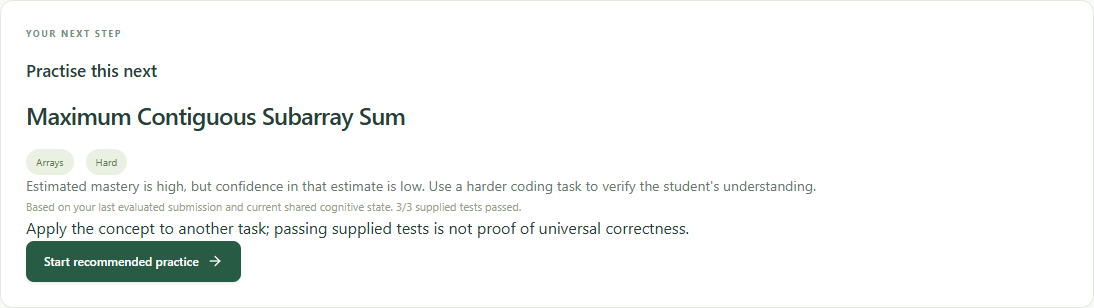
\includegraphics[width=0.98\textwidth,keepaspectratio]{coding-next-detail.png}
\caption{State-aware next-practice card after an actual fixture code assessment. Synthetic offline fixture; displayed performance is not a student-study result.}\label{fig:coding-next}
\end{figure}

\section{Worked Interaction and Interpretation}
A new profile requests an Arrays problem. With no assessed attempts, the policy begins at easy. The student submits a function, the runner checks supplied cases and the evaluator records the original result. If the code fails a boundary case, the recommendation can identify that case and retain a suitable level for revision. If a corrected original submission is accepted later, the next recommendation uses the updated state.

This example illustrates the agentic loop: observation changes the next action. It does not guarantee that the next problem is always harder, always newly generated or always on a different concept. Current coding recommendations stay within the assessed topic, and a targeted retry intentionally reuses the task when that is the supported response.

\chapter{Research Agent and Source-Grounded Reporting}\section{Introduction}
The Research Agent supports academic discovery, reading and source-based writing. Its role is to help the student work with papers, not to create the appearance of a completed literature review from titles alone. The current web workflow combines legitimate academic records, uploaded PDF text, persistent collections and coverage-aware exports.

This chapter distinguishes the wider research service architecture from the actions exposed in the student workspace. The project contains planning and bounded search components, but ordinary collection processing remains explicitly initiated in bounded batches. It should not be described as an unrestricted background researcher that downloads and analyses every available paper without supervision.

\section{Academic Topic Search}
The academic-search abstraction currently uses OpenAlex as its primary working provider. A search request returns real records where available: title, authors, publication year, abstract, DOI and source link. The application does not substitute generated paper identities when a provider returns fewer suitable records or fails.

A search target is a requested count, not a promise. Incremental retrieval can obtain further records within configured bounds, and the interface reports a shortfall when fewer valid papers are available. The previous arbitrary five-paper restriction is not imposed on the current collection interface. Safety limits still exist and are displayed rather than hidden.

Search records are de-duplicated through existing source-identity logic before they are added to a profile-owned collection. A duplicate provider result should not appear as a new independent paper. Provider errors remain visible so that a short result list is not mistaken for a complete survey of the field.

\section{Persistent Mixed-Source Collections}
The student can select individual search results and retain them alongside uploaded PDFs. These source types carry different evidence coverage. A retrieved abstract may establish the broad purpose of a paper but omit its full method, dataset or limitations. An uploaded PDF can provide much more text, although extraction and selected-chunk processing may still leave gaps.

Table~\ref{tab:source-scopes} makes this distinction explicit. The system preserves the source's identity and coverage instead of promoting an abstract to full-text status because it was added to a collection.
\begin{table}[htbp]\centering\small
\caption{Source coverage in the research workflow}\label{tab:source-scopes}
\begin{tabular}{P{0.23\textwidth}P{0.32\textwidth}P{0.35\textwidth}}\toprule
Source form & Available evidence & Required qualification\\\midrule
Academic search record & Provider metadata and available abstract & Abstract-only analysis; unavailable details stay missing.\\
Extracted uploaded PDF & Text associated with pages and chunks & Full-text excerpts; extraction and processing coverage disclosed.\\
Scanned or text-poor PDF & Insufficient usable extracted text & OCR is unavailable; do not fabricate an analysis.\\
Partially processed source & Completed chunks and recoverable errors & Explicit partial coverage, not a complete analysis.\\\bottomrule
\end{tabular}
\end{table}

Collections are stored by student profile. Search selections, uploaded documents, extraction records and supported analysis state recover through the database. This persistence supports continuity after refresh or restart. It does not authorise the system to mix one student's uploaded paper with another student's collection.

\section{PDF Extraction and Safety Limits}
The extractor processes actual PDF bytes and obtains text using the existing PDF extraction path. It does not infer the contents from a filename. Uploaded documents are checked for duplicates, and invalid or corrupted files retain a recoverable error status. Extraction runs through a worker with time and resource bounds rather than allowing an unbounded request to block indefinitely.

The default limits include 20 MiB per PDF, 100 documents per collection, 200 MiB collection storage, 300 pages per document and one million extracted characters. Chunk size defaults to 10,000 characters, extraction processes up to three pending documents in a batch, and analysis processes up to six pending chunks in a batch. These values come from the source defaults and can be overridden through the configured environment fields.

These bounds are operational safeguards, not recommended sample sizes for academic research. A collection with more than five papers is supported, subject to the configured limits. Conversely, a large successful upload does not mean every page has already been analysed. The interface must show the difference between stored, extracted and analysed content.

Image-only papers remain a limitation because OCR is not implemented. Tables, mathematical notation and multi-column layouts can also be extracted imperfectly. Source context must therefore be inspected when a reported finding depends on exact numerical or structural detail.

\section{Chunk Analysis and Provenance}
The full-text analysis path divides extracted text into attributable chunks and requests structured analysis from the provider. Supported fields include overview, research problem, objectives, methodology, dataset, experimental setup, models or algorithms, evaluation information, findings and limitations. A field can remain unavailable when its supporting content is absent.

Accepted claims retain a quotation and the originating page or chunk identity. The source quote is checked against the available material. This provides an auditable connection between a report statement and the text used to support it. A saved AI interpretation remains distinguishable from the exact quotation.

Quotation matching does not establish every aspect of scientific validity. A sentence may describe related work, a future proposal or an author's own experiment. A correctly copied sentence can still be assigned to the wrong role. The report therefore uses conservative labels and warns that method roles and findings may require checking in context.

\begin{figure}[htbp]\centering
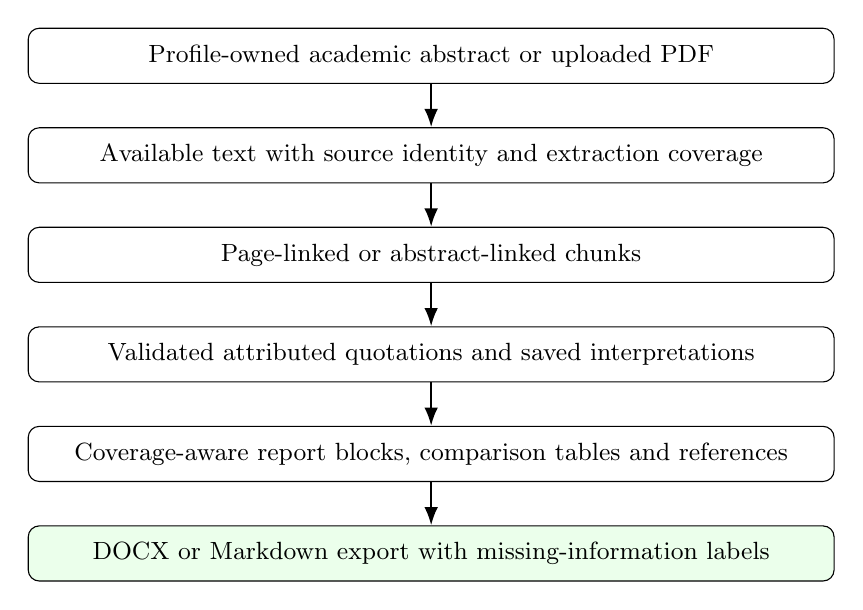
\begin{tikzpicture}[node distance=0.55cm,box/.style={draw,rounded corners,align=center,font=\small,text width=10.0cm,minimum height=0.7cm},arr/.style={-{Latex},thick}]
\node[box](source){Profile-owned academic abstract or uploaded PDF};
\node[box,below=of source](text){Available text with source identity and extraction coverage};
\node[box,below=of text](chunk){Page-linked or abstract-linked chunks};
\node[box,below=of chunk](claim){Validated attributed quotations and saved interpretations};
\node[box,below=of claim](report){Coverage-aware report blocks, comparison tables and references};
\node[box,below=of report,fill=green!8](export){DOCX or Markdown export with missing-information labels};
\draw[arr](source)--(text);\draw[arr](text)--(chunk);\draw[arr](chunk)--(claim);\draw[arr](claim)--(report);\draw[arr](report)--(export);
\end{tikzpicture}
\caption{Research evidence pipeline. Missing text cannot be replaced by an invented source claim.}\label{fig:research-pipeline}
\end{figure}

\section{Report Preparation and Readiness}
The web layer checks whether selected sources have usable completed analysis before enabling an ordinary analysis report. Readiness considers selected sources, available and processed chunks, supported claims, extraction status and failures. A selected collection without accepted analysis is not treated as a completed review.

The student can prepare another bounded batch, retry a failure or exclude an unusable source. A partial report requires an explicit choice and retains its partial-coverage label. A metadata-only bibliography is a separate option and cannot be represented as a methodology or findings report.

This readiness layer was added because a report can be syntactically valid while academically unhelpful. A Word document with headings and repeated ``not available'' messages may open correctly, yet it does not contain completed analysis. The workflow now makes that distinction before export and preserves the reason for incomplete coverage.

\section{Selectable Report Sections}
The report supports a title and topic, analysed paper details and references, individual overviews, objectives, methodologies, dataset and evaluation information, a methodology comparison table, thematic synthesis, similarities and differences, preliminary gaps, future directions, and limitations with source coverage.

Selecting a section is not permission to invent its content. When the analysed excerpts do not contain a dataset name or evaluation protocol, the document states that the information is unavailable in that coverage. An absent mention is not evidence that the original paper used no dataset or performed no evaluation.

The current web writer builds connected narrative from attributed saved evidence. Conservative lexical checks can reuse a supported span in an appropriate dataset or metric field when its cues are explicit. These checks are report aids, not independent semantic review. The generated report is not presented as a systematic literature review.

\section{Observations, Comparisons and Suggestions}
A comparison table can place available method excerpts side by side without establishing which method is better. Papers may use different datasets, metrics or experimental conditions. The report should not infer a common benchmark or a meaningful numerical ranking when none has been established.

Source-supported observations are separated from system suggestions. A preliminary gap can suggest that an issue deserves investigation, but the uploaded collection may be too small or incomplete to prove novelty. Future directions are therefore labelled as proposals requiring verification against wider literature and practical feasibility.

This restraint is a deliberate trade-off. It may produce a shorter report than unconstrained generation, but the text remains connected to material the application actually processed. A human researcher can expand the report after checking the sources rather than first having to remove fabricated citations and results.

\section{DOCX and Markdown Export}
The Word export uses python-docx to produce a real Office Open XML document with headings, paragraphs, tables and references. The Markdown export remains available. In the web application, a shared report-block model helps keep the two formats aligned so that one format does not silently introduce unsupported content missing from the other.

References use available metadata and stable source identity. PDF claims retain page or chunk references, while retrieved abstracts keep their abstract-only labels. Missing authors, years or DOI values remain missing. The report's readability is improved through organisation and attribution, rather than by filling every empty section with generated academic language.

\section{Research Comprehension and CACM}
Searching, uploading, extraction, analysis and export do not update mastery. They are actions performed by the system. The separate research-comprehension workflow can generate a question from supported analysed material and evaluate the student's actual answer. That accepted assessment can be adapted into CACM evidence.

This is the Research Agent's educational connection to the shared cognitive model. A student who downloads a polished report has not necessarily understood its sources. Requiring an evaluated interpretation keeps the system's analysis capability separate from the student's demonstrated understanding.

\section{Agentic Behaviour in the Research Workflow}
The agentic contribution is the coordinated choice and execution of relevant research actions, observation of their statuses and recovery when they fail. A query can enter actual academic search or a saved collection. Bounded planning services support focused research goals, while the web workflow preserves explicit source selection and processing controls.

The feedback loop is constrained by evidence availability. A failed extraction changes the next useful action to retrying or replacing the source. An incomplete collection requires more processing or a labelled partial export. A comprehension assessment can change the student's cognitive state. None of these operations justifies claiming that the system independently establishes scientific novelty or guarantees a complete literature review.

\chapter{System Validation and Results}\section{Introduction}
Evaluation was directed at the application's operational claims: entering the correct workflow, preserving student ownership, applying assessment evidence once, retaining source coverage and recovering saved work. These claims can be checked with deterministic tests. Educational effectiveness requires a different form of evaluation and is not inferred from software-test success.

The results reported here concern the web application at the coding next-practice implementation baseline, commit \module{40e5a88}. The original development reports are retained in the repository. A further offline backend run was performed during thesis preparation, with its machine-readable output included in the accompanying evidence directory. The thesis-preparation rerun passed all 77 backend tests in 52.20 seconds and all nine selected browser tests in 26.6 seconds, including two dashboard checks. These overlap with the baseline suites and are not additional independent performance samples. Test executions are not student participants, and multiple test layers are not combined into an educational accuracy percentage.

\section{Evaluation Setup}
The backend suite uses temporary SQLite stores, synthetic profiles and controlled replacements at external provider boundaries. The real application service, cognitive state, persistence and supported code-execution paths remain in use. External network access is denied in these tests apart from the local addresses needed by the harness.

Browser checks run the built React application against an explicit offline fixture server. Chrome automation interacts with actual controls, including Monaco code editing, submission buttons, topic selection and refresh. The fixture server substitutes predictable semantic routes, academic results and model responses. Consequently, these tests check application integration around the providers, not the live providers' ability to understand every arbitrary request.

No paid live-provider run was used to support the results in Table~\ref{tab:test-results}. No real-student dataset, learning-gain experiment, usability questionnaire or longitudinal assessment is reported.

\section{Recorded Test Results}
\begin{table}[htbp]\centering\small
\caption{Executed verification recorded for the implementation baseline}\label{tab:test-results}
\begin{tabular}{P{0.47\textwidth}P{0.18\textwidth}P{0.25\textwidth}}\toprule
Verification & Result & Interpretation\\\midrule
Backend API and service regression suite & 77 passed & Includes 11 next-practice tests.\\
Existing open-topic coding suite & 16 executions passed & Generated-package compatibility.\\
Existing verified coding catalogue suite & 10 executions passed & Supplied exercise contracts.\\
Existing persistence suite & 8 executions passed & Supported state recovery.\\
Selected browser regression run & 7 passed & Actual interface interactions with fixtures.\\
Final recommendation-browser recheck & 1 passed again & Repeat of one scenario, not a new independent case.\\
Thesis-preparation browser rerun & 9 passed & Includes the seven paths and two dashboard checks.\\
TypeScript and production frontend build & Passed & Build validity, not educational effectiveness.\\\bottomrule
\end{tabular}
\end{table}

The backend run reported one existing Starlette/httpx deprecation warning. The frontend build reported the existing large Monaco-related chunk warning. Neither warning was hidden or represented as a failed functional test. The entire browser suite was not executed for the feature baseline, so no claim is made that every historical browser test passed.

\section{Routing and Actual Workflow Entry}
Tests verify that a learning request prepares a lesson and practice controls, a coding request prepares a real exercise package and editor, and a research request enters search or collection functionality. An ambiguous request preserves a contextual clarification without executing an unrelated specialist.

The direct agent buttons are also exercised. They remain alternative entry points to the existing services. Their presence does not remove the common input, and moving between them must not erase another topic's supported unfinished quiz or introduce a separate cognitive record.

These results support the claim that the interface is connected to backend workflows. They do not measure the semantic router's accuracy on an independently sampled collection of student language. A live routing evaluation would require labelled requests and a specified scoring method.

\section{Learning-State and Quiz Validation}
The learning checks verify question identity, actual difficulty labels, topic binding and assessment recovery. Switching from Recursion to Arrays must not show the former topic's question as the latter topic's practice. Returning to an unfinished topic restores its supported session. Refresh retains the current question identifier and accepted evidence.

The tests also check that answering a question can update the student's assessed record, while opening the lesson or changing a topic does not. Repeated completed submissions remain idempotent. This validates a state-management property, not the pedagogical quality of every generated question or its scoring rubric.

\section{Coding Evaluation and Recommendation Validation}
The coding checks execute controlled original programs against actual supplied tests. They verify saved code, returned test outcomes, duplicate assessment protection and preservation of evidence when obtaining review feedback. Topic switching retains edited drafts instead of silently replacing them with new starter code.

The next-practice checks cover absence of recommendations before assessment, successful transition to a different verified task, focused retry after failure, stale and foreign-profile token rejection, process-restart recovery, provider failure, repeated candidate rejection and generated-variant validation. Pending assessment and standalone review do not produce ordinary practice recommendations. A genuine cross-agent conflict blocks normal next-practice start until the existing diagnostic path is used.

The browser scenario submits a correct Arrays solution, observes the recommendation, starts the actual policy-selected exercise and reloads the page. It compares saved student state and evidence before and after navigation. The key result is that opening the next task changes the activity but not mastery. Only a later evaluated student submission can provide new evidence.

\section{Research Reliability and Export Checks}
The backend research tests cover provider-response parsing, collections containing more than five sources, duplicate selections, profile isolation, actual PDF extraction and corrupted files. Report tests inspect readiness, partial coverage, references and the distinction between abstracts and full-text excerpts.

A valid DOCX must be an actual readable document structure rather than text renamed with a Word extension. Tests check the exported package and supported content. Truthfulness checks ensure that empty or unprocessed selections cannot be represented as a completed analysis report. These checks do not establish that the source papers themselves are correct or that every accepted quotation has been interpreted perfectly.

\section{Persistence and Refresh Recovery}
Recovery is tested at both service and browser levels. A fresh application instance using the same test database simulates process restart. Reloading the browser checks restoration of visible activity. Saved drafts, questions, collections, recommendation focus and accepted evidence are checked in the relevant scenarios.

These tests address an earlier weakness of in-memory-only interfaces: a browser refresh can create a new session unless important state has been committed to durable storage. PHSS now reconstructs supported state from profile-owned snapshots and research records. Recovery is bounded by what the codec and checkpoint paths actually save; it is not a claim that every arbitrary runtime object is serialised.

\section{Requirement-to-Evidence Traceability}
Table~\ref{tab:traceability} links major requirements to concrete verification areas. This makes the evaluation easier to audit than a single summary percentage.
\begin{longtable}{P{0.32\textwidth}P{0.59\textwidth}}
\caption{Requirement traceability for the implemented web system}\label{tab:traceability}\\
\toprule Requirement & Verification area\\\midrule\endfirsthead
\toprule Requirement & Verification area\\\midrule\endhead
Automatic workflow entry & Backend route fixtures; browser agent-entry and workspace checks.\\
Topic-specific adaptive quiz & Learning-topic backend tests and learning-quiz browser scenario.\\
Original code assessment & Real runner tests, submission API and browser editor interaction.\\
Evidence-based next practice & Eleven recommendation tests and browser transition/recovery scenario.\\
Persistent research collection & Search, upload, duplicate and profile-isolation API tests.\\
Grounded report readiness & Report flow, truthfulness, synthesis and reliability test modules.\\
No mastery for navigation/generation & Evidence comparisons before and after non-assessment operations.\\
Refresh and restart recovery & New service instance with the same test database; browser reload checks.\\
Provider failure recovery & Controlled provider errors and retained original work.\\
\bottomrule
\end{longtable}

\section{Discussion of Agentic Behaviour}
The strongest evidence for agentic behaviour is the connection between observation and action. The system does not simply label a response ``Coding Agent.'' It invokes code-evaluation services and uses the result to choose a subsequent activity. Likewise, the research workflow observes extraction and analysis status before deciding whether an export is ready, partial or unavailable.

This evidence supports a bounded hybrid-agentic description. Rule-based control is part of the design, and the student remains involved at assessment boundaries. No numerical ``agentic percentage'' is reported because there is no defined measurement method for dividing UI, persistence, policies and model calls into such a percentage.

\section{Limitations and Threats to Validity}
Controlled fixtures improve reproducibility but reduce exposure to live-provider variability. They cannot measure current search completeness, arbitrary topic support or the reliability of a changing model endpoint. The selected browser suite also covers representative paths rather than every possible interaction ordering.

The mastery rule, confidence accumulation and difficulty thresholds have not been calibrated against real student outcomes. No control group, pre-test/post-test design or retention study was conducted. This prevents claims of demonstrated learning improvement, fairness across student groups or a validated mastery probability.

Operational limits also remain. Local profiles are not secure authentication; Python execution is not a hardened public sandbox; PDF OCR is unavailable; and quotation validation cannot independently prove scientific interpretation. Load testing, accessibility auditing and a public multi-user security assessment remain future work. These limitations should accompany demonstrations rather than be concealed by the successful test counts.

\chapter{Conclusion and Scope for Further Research}\section{Summary of the Work}
CACM-PHSS was developed as a web-based study environment in which conceptual learning, coding practice and research reading share a student evidence model. The React interface provides a common natural-language entry point, while FastAPI connects it to the existing Python orchestration and specialist services. SQLite persistence retains supported activity state and research collections across refresh and restart.

The project moved from an initial Streamlit testing interface to the present web application. The thesis concentrates on the web system and its real workflows rather than treating the prototype and web frontend as separate educational methods.

\section{Principal Findings}
The implementation demonstrates that the three specialist activities can be entered from one interface without requiring a manual agent choice. The same services remain accessible through direct buttons. Shared evidence allows a later activity to read the student's existing concept state, and disagreement can trigger a focused diagnostic rather than being hidden.

The coding next-practice feature provides a concrete example of bounded replanning. It observes an original assessment, selects revision or further practice and preserves the reason across navigation and refresh. Research processing provides another example: export eligibility depends on actual source analysis and failures, not merely on a request to generate a report.

Recorded backend, selected existing-suite and browser checks support these operational findings under deterministic offline fixtures. They do not establish educational superiority or live-provider performance for arbitrary topics.

\section{Contributions}
The main contribution is the integration of specialist workflows with explicit evidence boundaries. Content generation, code correction, paper analysis and report export are useful system actions, but they are not treated as student mastery. Assessment receipts, profile ownership and durable snapshots preserve this distinction over repeated and interrupted operations.

A second contribution is honest source coverage in research support. Retrieved abstracts, extracted full-text excerpts and incomplete processing remain distinguishable. The report writer can organise available evidence without claiming that missing methodological detail has been found.

\section{Scope and Limitations}
The present application is a local prototype with practical engineering safeguards. Its cognitive policy is rule-based. Its confidence value is not a calibrated probability, and its correctness judgements remain limited by supplied tests and provider feedback. It has not been evaluated through a real-student study.

These boundaries mean that the application is best presented as an implemented multi-agent personalised study platform with reproducible software verification. It should not be described as a fully autonomous teacher, a secure public code-execution service or a validated replacement for academic supervision.

\section{Scope for Further Research}
A future educational study could compare appropriately matched study conditions using pre-tests, post-tests and delayed retention measures. Such a study would require consent, an ethical data-handling plan and clearly defined outcomes. Calibration work could compare the current estimates with subsequent independently scored responses before changing the mastery policy.

Further engineering work could add authenticated accounts, stronger execution isolation, accessibility testing and measured concurrency limits. OCR and richer document-layout handling could improve source coverage. Research suggestions could be strengthened by broader verified retrieval, while preserving the separation between source observations and proposed directions.

Cross-topic coding recommendations are another possible extension. They would require a defensible relationship between concepts and additional checks that prerequisite suggestions are appropriate. None of these future directions is counted as a completed feature in this thesis.

\appendix
\chapter{Implementation Parameters, Reproducibility and Additional Tables}
\section{Implementation Baseline}
The implementation described in this thesis was inspected in the separate PHSS web-application project. Its source baseline is commit \module{40e5a88} on branch \module{phss-web-app}. Thesis-only changes follow that baseline. The application repository is \url{https://github.com/Shaswathisanjana/Personalized-Hybrid-Study-System}.

The frontend uses React components~\cite{reactdocs} and TypeScript, built with Vite. FastAPI~\cite{fastapidocs} exposes the Python services, and Uvicorn runs the local server. PDF extraction uses pypdf~\cite{pypdfdocs}, academic retrieval uses the existing OpenAlex provider~\cite{openalexdocs}, and Word export uses python-docx~\cite{docxdocs}. These citations identify supporting tools; they do not imply that their maintainers endorse the project.

\section{Source Traceability}
\begin{longtable}{P{0.37\textwidth}P{0.54\textwidth}}
\caption{Principal implementation locations used in the thesis}\label{tab:source-map}\\
\toprule Area & Source location\\\midrule\endfirsthead
\toprule Area & Source location\\\midrule\endhead
HTTP routes and input validation & \module{backend/main.py}\\
Workflow integration & \module{backend/service.py}\\
Semantic routing and clarification & \module{app/orchestrator/query_router.py}\\
Bounded workspace and advancement & \module{app/orchestrator/study_workspace.py}\\
Shared student model & \module{app/cognitive/models.py}\\
Mastery update & \module{app/cognitive/mastery_engine.py}\\
Cross-agent conflicts & \module{app/cognitive/conflict_detector.py}\\
Assessment evidence integration & \module{app/cognitive/cognitive_engine.py}\\
Adaptive learning question policy & \module{app/learning_agent/practice_policy.py}\\
Topic-specific web practice binding & \module{backend/practice_context.py}\\
Coding action policy & \module{app/coding_agent/agent.py}\\
Coding execution and evaluation & \module{app/coding_agent/evaluator.py}\\
Generated coding package validation & \module{app/coding_agent/open_topic.py}\\
Coding follow-up recommendation & \module{backend/coding_recommendations.py}\\
PDF collection bounds & \module{app/research_agent/collection_models.py}\\
Research processing & \module{app/research_agent/collection_service.py}\\
Web report readiness and writing & \module{backend/research_reports.py}\\
Conservative report synthesis & \module{backend/report_synthesis.py}\\
Profile snapshots and research storage & \module{app/persistence/sqlite_store.py}\\
Supported session recovery & \module{app/persistence/session_recovery.py}\\
Student interface & \module{frontend/src/App.tsx}\\\bottomrule
\end{longtable}

\section{Default PDF Processing Parameters}
\begin{table}[htbp]\centering\small
\caption{Source defaults for PDF collection processing}\label{tab:pdf-defaults}
\begin{tabular}{P{0.54\textwidth}P{0.34\textwidth}}\toprule
Parameter & Default\\\midrule
Maximum single PDF size & 20 MiB\\
Maximum documents & 100\\
Maximum collection bytes & 200 MiB\\
Maximum PDF pages & 300\\
Maximum extracted characters & 1,000,000\\
Chunk characters & 10,000\\
Minimum usable text characters & 80\\
Documents extracted per batch & 3\\
Chunks analysed per batch & 6\\
Extraction timeout & 45 seconds\\
Provider timeout field & 60 seconds\\
Worker memory limit field & 512 MiB\\\bottomrule
\end{tabular}
\end{table}
These are configured defaults rather than universal platform guarantees. Environment overrides and operating-system support affect runtime behaviour. They should be checked in the application's displayed settings when reproducing an execution.

\section{Reproducing Offline Verification}
From the web-application root, the backend regression command is:
\begin{verbatim}
.\.venv\Scripts\python.exe -B -m pytest backend/tests -q
\end{verbatim}
Selected existing suites are run through \module{tools/evaluate_offline.py} with the exact case names \module{test_open_topic_coding}, \module{test_verified_coding_catalog} and \module{test_persistence_streamlit}. The last name reflects the history of a shared recovery test suite; it is not an evaluation of a second primary application in this thesis.

The frontend build command is \texttt{npm.cmd --prefix frontend run build}. From the frontend directory, Playwright can run the selected files \module{coding-recommendations.spec.ts}, \module{coding-workflow.spec.ts}, \module{learning-quiz.spec.ts}, \module{loading.spec.ts}, \module{agent-buttons.spec.ts} \module{topic-options.spec.ts} and \module{progress.spec.ts}. The offline fixture server is configured in \module{frontend/playwright.config.ts}.

\section{Demonstration Procedure}
A demonstration can begin with ``Teach me recursion,'' continue to an adaptive answer, and show the explicit question difficulty. A second request can ask for an Arrays coding problem. After an original submission is evaluated, the presenter can inspect its supplied-test outcomes and next-practice recommendation. Refresh should recover the saved activity.

For research, the presenter can request academic papers, select results or upload usable PDFs, process a bounded batch and inspect analysis readiness before export. The demonstration must identify whether it uses controlled fixtures or live providers. Fixture screenshots illustrate interface behaviour and must not be presented as results from real students.

\section{Submission Checklist}
Before formal submission, confirm the final approved title, guide's name, authorised countersignatory, examination date, institutional logo and required declaration wording. Review every chapter against the final code baseline. Verify the reference formatting in the compiled PDF, replace any remaining metadata placeholders and obtain institutional approval for the certificate text.

A similarity checker has not been run as part of this preparation. Original project-specific wording and citations reduce inappropriate copying, but no fixed similarity percentage can be guaranteed. The team remains responsible for reviewing the work, acknowledging permitted assistance and following its institution's submission policy.

\clearpage
\renewcommand{\bibname}{References}
\phantomsection\addcontentsline{toc}{chapter}{References}
\bibliographystyle{ieeetr}
\bibliography{mybib}
\chapter*{List of Publications \\ \large(Based on the Research Work)}
\addcontentsline{toc}{chapter}{List of Publications Based on the Research Work}
Publication details have not been provided for this draft. The project team must confirm the publication status before submission. No publication claim is made here.
\end{document}
